\documentclass[onlymath]{beamer}
% \documentclass[onlymath,handout]{beamer}

% Macros used by all lectures, but not necessarily by excercises

%%% General setup and dependencies:

% \usetheme[ddcfooter,nosectionnum]{tud}
\usetheme[nosectionnum,pagenum,noheader]{tud}
% \usetheme[nosectionnum,pagenum]{tud}

% Increase body font size to a sane level:
\let\origframetitle\frametitle
% \renewcommand{\frametitle}[1]{\origframetitle{#1}\normalsize}
\renewcommand{\frametitle}[1]{\origframetitle{#1}\fontsize{10pt}{13.2}\selectfont}
\setbeamerfont{itemize/enumerate subbody}{size=\small} % tud defaults to scriptsize!
\setbeamerfont{itemize/enumerate subsubbody}{size=\small}
% \setbeamerfont{normal text}{size=\small}
% \setbeamerfont{itemize body}{size=\small}

\renewcommand{\emph}[1]{\textbf{#1}}

\def\arraystretch{1.3}% Make tables even less cramped vertically

\usepackage[ngerman]{babel}
\usepackage[utf8]{inputenc}
\usepackage[T1]{fontenc}

%\usepackage{graphicx}
\usepackage[export]{adjustbox} % loads graphicx
\usepackage{import}
\usepackage{stmaryrd}
\usepackage[normalem]{ulem} % sout command
% \usepackage{times}
\usepackage{txfonts}

% \usepackage[perpage]{footmisc} % reset footnote counter on each page -- fails with beamer (footnotes gone)
\usepackage{perpage}  % reset footnote counter on each page
\MakePerPage{footnote}

\usepackage{tikz}
\usetikzlibrary{arrows,positioning}
% Inspired by http://www.texample.net/tikz/examples/hand-drawn-lines/
\usetikzlibrary{decorations.pathmorphing}
\pgfdeclaredecoration{penciline}{initial}{
    \state{initial}[width=+\pgfdecoratedinputsegmentremainingdistance,
    auto corner on length=1mm,]{
        \pgfpathcurveto%
        {% From
            \pgfqpoint{\pgfdecoratedinputsegmentremainingdistance}
                      {\pgfdecorationsegmentamplitude}
        }
        {%  Control 1
        \pgfmathrand
        \pgfpointadd{\pgfqpoint{\pgfdecoratedinputsegmentremainingdistance}{0pt}}
                    {\pgfqpoint{-\pgfdecorationsegmentaspect
                     \pgfdecoratedinputsegmentremainingdistance}%
                               {\pgfmathresult\pgfdecorationsegmentamplitude}
                    }
        }
        {%TO 
        \pgfpointadd{\pgfpointdecoratedinputsegmentlast}{\pgfpoint{1pt}{1pt}}
        }
    }
    \state{final}{}
}
\tikzset{handdrawn/.style={decorate,decoration=penciline}}
\tikzset{every shadow/.style={fill=none,shadow xshift=0pt,shadow yshift=0pt}}
% \tikzset{module/.append style={top color=\col,bottom color=\col}}

% Use to make Tikz attributes with Beamer overlays
% http://tex.stackexchange.com/a/6155
\tikzset{onslide/.code args={<#1>#2}{%
  \only<#1| handout:0>{\pgfkeysalso{#2}} 
}}
\tikzset{onslideprint/.code args={<#1>#2}{%
  \only<#1>{\pgfkeysalso{#2}} 
}}

%%% Title -- always set this first

\newcommand{\defineTitle}[3]{
	\newcommand{\lectureindex}{#1}
	\title{Formale Systeme}
	\subtitle{\href{\lectureurl}{#1. Vorlesung: #2}}
	\author{\href{http://korrekt.org/}{Markus Kr\"{o}tzsch}}
%	\author{\href{http://www.sebastian-rudolph.de}{Sebastian Rudolph} in Vertretung von \href{http://korrekt.org/}{Markus Kr\"{o}tzsch}}
	\date{#3}
	\datecity{TU Dresden}
% 	\institute{Computational Logic}
}

%%% Table of contents:

\RequirePackage{ifthen}

\newcommand{\highlight}[2]{%
	\ifthenelse{\equal{#1}{\lectureindex}}{\alert{#2}}{#2}%
}

\def\myspace{-0.7ex}
\newcommand{\printtoc}{
\begin{tabular}{r@{$\quad$}l}
\highlight{1}{1.} & \highlight{1}{Willkommen/Einleitung formale Sprachen}\\[\myspace]
\highlight{2}{2.} & \highlight{2}{Grammatiken und die Chomsky-Hierarchie}\\[\myspace]
\highlight{3}{3.} & \highlight{3}{Endliche Automaten}\\[\myspace]
\highlight{4}{4.} & \highlight{4}{Complexity of FO query answering}\\[\myspace]
\highlight{5}{5.} & \highlight{5}{Conjunctive queries}\\[\myspace]
\highlight{6}{6.} & \highlight{6}{Tree-like conjunctive queries}\\[\myspace]
\highlight{7}{7.} & \highlight{7}{Query optimisation}\\[\myspace]
\highlight{8}{8.} & \highlight{8}{Conjunctive Query Optimisation / First-Order~Expressiveness}\\[\myspace]
\highlight{9}{9.} & \highlight{9}{First-Order~Expressiveness / Introduction to Datalog}\\[\myspace]
\highlight{10}{10.} & \highlight{10}{Expressive Power and Complexity of Datalog}\\[\myspace]
\highlight{11}{11.} & \highlight{11}{Optimisation and Evaluation of Datalog}\\[\myspace]
\highlight{12}{12.} & \highlight{12}{Evaluation of Datalog (2)}\\[\myspace]
\highlight{13}{13.} & \highlight{13}{Graph Databases and Path Queries}\\[\myspace]
\highlight{14}{14.} & \highlight{14}{Outlook: database theory in practice}
\end{tabular}
}

\newcommand{\overviewslide}{%
\begin{frame}\frametitle{Overview}
\printtoc
\medskip

Siehe \href{\lectureurl}{course homepage [$\Rightarrow$ link]} for more information and materials
\end{frame}
}

%%% Colours:

\usepackage{xcolor,colortbl}
\definecolor{redhighlights}{HTML}{FFAA66}
\definecolor{lightblue}{HTML}{55AAFF}
\definecolor{lightred}{HTML}{FF5522}
\definecolor{lightpurple}{HTML}{DD77BB}
\definecolor{lightgreen}{HTML}{55FF55}
\definecolor{darkred}{HTML}{CC4411}
\definecolor{darkblue}{HTML}{176FC0}%{1133AA}
\definecolor{nightblue}{HTML}{2010A0}%{1133AA}
\definecolor{alert}{HTML}{176FC0}
\definecolor{darkgreen}{HTML}{36AB14}
\definecolor{strongyellow}{HTML}{FFE219}
\definecolor{devilscss}{HTML}{666666}

\newcommand{\redalert}[1]{\textcolor{darkred}{#1}}

%%% Style commands

\newcommand{\quoted}[1]{\texttt{"}{#1}\texttt{"}}
\newcommand{\squote}{\texttt{"}} % straight quote
\newcommand{\Sterm}[1]{\ensuremath{\mathtt{\textcolor{purple}{#1}}}}    % letters in alphabets
\newcommand{\Snterm}[1]{\textsf{\textcolor{darkblue}{#1}}} % nonterminal symbols
\newcommand{\Sntermsub}[2]{\Snterm{#1}_{\Snterm{#2}}} % nonterminal symbols
\newcommand{\Slang}[1]{\textbf{\textcolor{black}{#1}}}    % languages
\newcommand{\Slangsub}[2]{\Slang{#1}_{\Slang{#2}}}    % languages
% Code
\newcommand{\Scode}[1]{\textbf{#1}}    % reserved words in program listings, e.g., "if"
\newcommand{\Scodelit}[1]{\textcolor{purple}{#1}}    % literals in program listings, e.g., strings
\newcommand{\Scomment}[1]{\textcolor{gray}{#1}}    % comment in program listings

\newcommand{\epstrastar}{\mathrel{\mathord{\stackrel{\epsilon}{\to}}{}^*}} % transitive reflexive closure of epsilon transitions in an epslion-NFA

\newcommand{\narrowcentering}[1]{\mbox{}\hfill#1\hfill\mbox{}}

\newcommand{\defeq}{\mathrel{:=}}

\newcommand{\Smach}[1]{\ensuremath{\mathcal{#1}}}    % machines

%%% Slide layout commands:

\newcommand{\sectionSlide}[1]{
\frame{\begin{center}
\LARGE
#1
\end{center}}
}
\newcommand{\sectionSlideNoHandout}[1]{
\frame<handout:0>{\begin{center}
\LARGE
#1
\end{center}}
}

\newcommand{\mydualbox}[3]{%
 \begin{minipage}[t]{#1}
 \begin{beamerboxesrounded}[upper=block title,lower=block body,shadow=true]%
    {\centering\usebeamerfont*{block title}#2}%
    \raggedright%
    \usebeamerfont{block body}
%     \small
    #3%
  \end{beamerboxesrounded}
  \end{minipage}
}
% 
\newcommand{\myheaderbox}[2]{%
 \begin{minipage}[t]{#1}
 \begin{beamerboxesrounded}[upper=block title,lower=block title,shadow=true]%
    {\centering\usebeamerfont*{block title}\rule{0pt}{2.6ex} #2}%
  \end{beamerboxesrounded}
  \end{minipage}
}

\newcommand{\mycontentbox}[2]{%
 \begin{minipage}[t]{#1}%
 \begin{beamerboxesrounded}[upper=block body,lower=block body,shadow=true]%
    {\centering\usebeamerfont*{block body}\rule{0pt}{2.6ex}#2}%
  \end{beamerboxesrounded}
  \end{minipage}
}

\newcommand{\mylcontentbox}[2]{%
 \begin{minipage}[t]{#1}%
 \begin{beamerboxesrounded}[upper=block body,lower=block body,shadow=true]%
    {\flushleft\usebeamerfont*{block body}\rule{0pt}{2.6ex}#2}%
  \end{beamerboxesrounded}
  \end{minipage}
}

% label=180:{\rotatebox{90}{{\footnotesize\textcolor{darkgreen}{Beispiel}}}}
% \hspace{-8mm}\ghost{\raisebox{-7mm}{\rotatebox{90}{{\footnotesize\textcolor{darkgreen}{Beispiel}}}}}\hspace{8mm}
\newcommand{\examplebox}[1]{%
	\begin{tikzpicture}[decoration=penciline, decorate]
		\pgfmathsetseed{1235}
		\node (n1) [decorate,draw=darkgreen, fill=darkgreen!10,thick,align=left,text width=\linewidth, inner ysep=2mm, inner xsep=2mm] at (0,0) {#1};
% 		\node (n2) [align=left,text width=\linewidth,inner sep=0mm] at (n1.92) {{\footnotesize\raisebox{3mm}{\textcolor{darkgreen}{Beispiel}}}};
% 		\node (n2) [decorate,draw=darkgreen, fill=darkgreen!10,thick, align=left,text width=\linewidth,inner sep=2mm] at (n1.90) {{\footnotesize\raisebox{0mm}{\textcolor{darkgreen}{Beispiel}}}};
	\end{tikzpicture}%
}%

\newcommand{\codebox}[1]{%
	\begin{tikzpicture}[decoration=penciline, decorate]
		\pgfmathsetseed{1236}
		\node (n1) [decorate,draw=strongyellow, fill=strongyellow!10,thick,align=left,text width=\linewidth, inner ysep=2mm, inner xsep=2mm] at (0,0) {#1};
	\end{tikzpicture}%
}%

\newcommand{\defbox}[1]{%
	\begin{tikzpicture}[decoration=penciline, decorate]
		\pgfmathsetseed{1237}
		\node (n1) [decorate,draw=darkred, fill=darkred!10,thick,align=left,text width=\linewidth, inner ysep=2mm, inner xsep=2mm] at (0,0) {#1};
	\end{tikzpicture}%
}%

\newcommand{\theobox}[1]{%
	\begin{tikzpicture}[decoration=penciline, decorate]
		\pgfmathsetseed{1240}
		\node (n1) [decorate,draw=darkblue, fill=darkblue!10,thick,align=left,text width=\linewidth, inner ysep=2mm, inner xsep=2mm] at (0,0) {#1};
	\end{tikzpicture}%
}%

\newcommand{\anybox}[2]{%
	\begin{tikzpicture}[decoration=penciline, decorate]
		\pgfmathsetseed{1240}
		\node (n1) [decorate,draw=#1, fill=#1!10,thick,align=left,text width=\linewidth, inner ysep=2mm, inner xsep=2mm] at (0,0) {#2};
	\end{tikzpicture}%
}%


\newsavebox{\mybox}%
\newcommand{\doodlebox}[2]{%
\sbox{\mybox}{#2}%
	\begin{tikzpicture}[decoration=penciline, decorate]
		\pgfmathsetseed{1238}
		\node (n1) [decorate,draw=#1, fill=#1!10,thick,align=left,inner sep=1mm] at (0,0) {\usebox{\mybox}};
	\end{tikzpicture}%
}%

% Common notation

\usepackage{amsmath,amssymb,amsfonts}
\usepackage{xspace}

\newcommand{\lectureurl}{https://iccl.inf.tu-dresden.de/web/FS2016}

\DeclareMathAlphabet{\mathsc}{OT1}{cmr}{m}{sc} % Let's have \mathsc since the slide style has no working \textsc

% Dual of "phantom": make a text that is visible but intangible
\newcommand{\ghost}[1]{\raisebox{0pt}[0pt][0pt]{\makebox[0pt][l]{#1}}}

\newcommand{\tuple}[1]{\langle{#1}\rangle}

%%% Annotation %%%

\usepackage{color}
\newcommand{\todo}[1]{{\tiny\color{red}\textbf{TODO: #1}}}



%%% Old macros below; move when needed

\newcommand{\blank}{\text{\textvisiblespace}} % empty tape cell for TM

% table syntax
\newcommand{\dom}{\textbf{dom}}
\newcommand{\adom}{\textbf{adom}}
\newcommand{\dbconst}[1]{\texttt{"#1"}}
\newcommand{\pred}[1]{\textsf{#1}}
\newcommand{\foquery}[2]{#2[#1]}
\newcommand{\ground}[1]{\textsf{ground}(#1)}
% \newcommand{\foquery}[2]{\{#1\mid #2\}} %% Notation as used in Alice Book
% \newcommand{\foquery}[2]{\tuple{#1\mid #2}}

\newcommand{\quantor}{\mathord{\reflectbox{$\text{\sf{Q}}$}}} % the generic quantor

% logic syntax
\newcommand{\Inter}{\mathcal{I}} %used to denote an interpretation
\newcommand{\Jnter}{\mathcal{J}} %used to denote another interpretation
\newcommand{\Knter}{\mathcal{K}} %used to denote yet another interpretation
\newcommand{\Zuweisung}{\mathcal{Z}} %used to denote a variable assignment

% query languages
\newcommand{\qlang}[1]{{\sf #1}} % Font for query languages
\newcommand{\qmaps}[1]{\textbf{QM}({\sf #1})} % Set of query mappings for a query language

%%% Complexities %%%

\hyphenation{Exp-Time} % prevent "Ex-PTime" (see, e.g. Tobies'01, Glimm'07 ;-)
\hyphenation{NExp-Time} % better that than something else

% \newcommand{\complclass}[1]{{\sc #1}\xspace} % font for complexity classes
\newcommand{\complclass}[1]{\ensuremath{\mathsc{#1}}\xspace} % font for complexity classes

\newcommand{\ACzero}{\complclass{AC$_0$}}
\newcommand{\LogSpace}{\complclass{L}}
\newcommand{\NLogSpace}{\complclass{NL}}
\newcommand{\PTime}{\complclass{P}}
\newcommand{\NP}{\complclass{NP}}
\newcommand{\coNP}{\complclass{coNP}}
\newcommand{\PH}{\complclass{PH}}
\newcommand{\PSpace}{\complclass{PSpace}}
\newcommand{\NPSpace}{\complclass{NPSpace}}
\newcommand{\ExpTime}{\complclass{ExpTime}}
\newcommand{\NExpTime}{\complclass{NExpTime}}
\newcommand{\ExpSpace}{\complclass{ExpSpace}}
\newcommand{\TwoExpTime}{\complclass{2ExpTime}}
\newcommand{\NTwoExpTime}{\complclass{N2ExpTime}}
\newcommand{\ThreeExpTime}{\complclass{3ExpTime}}
\newcommand{\kExpTime}[1]{\complclass{#1ExpTime}}
\newcommand{\kExpSpace}[1]{\complclass{#1ExpSpace}}


\defineTitle{3}{Endliche Automaten}{17. Oktober 2016}

\begin{document}

\maketitle

\sectionSlideNoHandout{Rückblick}

\begin{frame}\frametitle{Wiederholung}

Mit Grammatiken können wir Sprachen beschreiben und sie grob in Typen unterteilen:\medskip

\begin{tikzpicture}[decoration=penciline, decorate]
\node (nl) [decorate,draw=nightblue, text depth = 4cm, text width = \linewidth, fill=nightblue!10,thick,align=left, inner ysep=2mm, inner xsep=2mm] at (0,0) {Formale Sprachen};
\node (n0) [decorate,draw=darkgreen, text depth = 3cm, text width = 8cm, fill=darkgreen!10,thick,align=left, inner ysep=2mm, inner xsep=2mm] at ([yshift=-0.5em]nl.center) {Typ-0-Sprachen};
\node (n1) [decorate,draw=strongyellow, text depth = 2cm, text width = 6.7cm,  fill=strongyellow!10,thick,align=left, inner ysep=2mm, inner xsep=2mm] at ([yshift=-0.5em]n0.center) {Kontextsensitive Sprachen (Typ 1)};
\node (n2) [decorate,draw=orange, text depth = 1cm, text width = 5.4cm,  fill=orange!10,thick,align=left, inner ysep=2mm, inner xsep=2mm] at ([yshift=-0.5em]n1.center) {Kontextfreie Sprachen (Typ 2)};
\node (n3) [decorate,draw=red, fill=red!10,thick,align=left, inner ysep=2mm, inner xsep=2mm] at ([yshift=-0.5em]n2.center) {Reguläre Sprachen (Typ 3)};
\end{tikzpicture}

\end{frame}

% \sectionSlide{Grammatiken in der Praxis}

\begin{frame}\frametitle{Grammatiken in der Praxis}

Eine "`ASCII-Syntax"' für Typ-2-Grammatiken\\ ist die sogenannte \redalert{Backus-Naur-Form} (BNF):\footnote{Panini, 5./4. Jhd. v. Chr.; neu erfunden von John Backus in 1959}

\begin{itemize}
\item statt $\to$ wird \alert{$\mathtt{::=}$} verwendet 
\item \alert{$\mid$} für Alternativen (wie bei uns)
\item Markierung: \alert{\squote}Terminalsymbole\alert{\squote}\\
      und {\alert{$\texttt{<}$}Nichterminalsymbole\alert{$\texttt{>}$}}
\end{itemize}

\ghost{\hspace{7.2cm}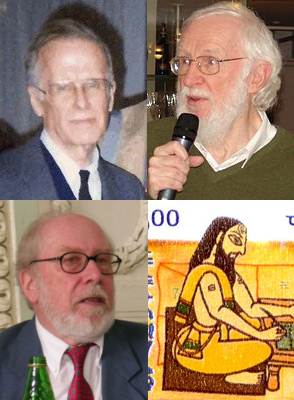
\includegraphics[width=3.5cm]{images/BNF-Autoren} ~\rotatebox{90}{{\tiny{oben: John Backus, Peter Naur}}} \rotatebox{90}{{\tiny{unten: Nicklas Wirth, Panini}}}}%
\pause\redalert{Erweiterte BNF} (EBNF, von Nicklas Wirth):
\begin{itemize}
\item allgemein wie BNF, aber Konkatenation mit Kommas
\item Zusätzliche Abkürzungen \alert{\texttt{[X]}} für "`null oder ein X"' und \alert{\texttt{\{X\}}} für "`null oder mehr X"'
% \item Es gibt weitere Versionen von "`EBNF"', z.B. verwendet das W3C eine eigene EBNF
% \item Es gibt noch mehr Erweiterungen von BNF, z.B. \emph{Augmented BNF} (ABNF), ein Standard der IETF
\end{itemize}

\alert{In der Praxis sind unterschiedliche Notationen im Einsatz}

{\footnotesize (EBNF von Wirth; ISO EBNF; W3C EBNF; "`Augmented BNF"' der IETF; verschiedene "`EBNF"' aus Vorlesungen und Lehrbüchern \ldots)}

\end{frame}


\sectionSlide{Sprachen Nutzen und Verstehen}


\begin{frame}\frametitle{Von Beschreiben zu Erkennen}

Grammatiken beschreiben Sprachen als Mengen von Wörtern, die sie \alert{erzeugen} können.
\medskip

Praktisch wichtige Aufgabe: \alert{erkenne} ob ein Wort in einer Sprache \ghost{liegt}

\defbox{
Das \redalert{Wortproblem} für eine Sprache $\Slang{L}$ über Alphabet $\Sigma$ besteht darin, die folgende Funktion zu berechnen:\\[1ex]
\emph{Eingabe:} ein Wort $w\in\Sigma^*$\\
\emph{Ausgabe:} "`ja"' wenn $w\in\Slang{L}$ und "`nein"' wenn $w\notin\Slang{L}$
}\pause

\examplebox{Für die Sprache $\{\Sterm{a}\}\circ \{\Sterm{b}\}^*$ wird das Wortproblem durch einen einfachen Algorithmus in linearer Zeit gelöst
(teste, ob der erste Buchstabe $\Sterm{a}$ ist und ob alle folgenden Buchstaben $\Sterm{b}$ sind).
}

Andererseits kann das Wortproblem sehr schwer sein, selbst für Sprachen, die mit einer Grammatik formal beschrieben sind.
% Für viele Grammatiken wird das Wortproblem nachweislich durch kein Computerprogramm gelöst.

\end{frame}

\begin{frame}\frametitle{Ausblick}

Wir werden sehen, dass jede Sprachklasse zu einem bestimmten Berechnungsmodell passt:
\bigskip

\begin{tabular}{@{}lll@{}}
\alert{Sprachklasse} & \alert{Berechnungsmodell} & \alert{Wortproblem}\\
Typ 0 & Turingmaschine (TM) & semi-entscheidbar\footnote{Akzeptanz von Wörtern kann beliebig lange dauern, so dass man nie weiß, ob sie noch passiert; Wörter können nur rekursiv aufgezählt werden}\\
Kontextsensitiv & nichtdeterministische TM & PSpace-vollständig\footnote{höchstwahrscheinlich schwerer als NP; jeder praktisch bekannte Algorithmus benötigt im Worst Case exponentiell viel Zeit}\\[-1ex]
	&  mit linearem Speicher & \\
Kontextfrei & nichtdeterministischer & polynomiell\\[-1ex]
	&  Kellerautomat & \\
Regulär & endlicher Automat & polynomiell\footnote{tatsächlich sogar noch viel einfacher als Typ 2}
\end{tabular}
% 
% ndet. = nichtdeterministisch (dazu später mehr)

\end{frame}

\begin{frame}\frametitle{Weitere Fragestellungen}

Das Wortproblem ist nicht die einzige praktische relevante Frage.
\medskip

\alert{Darstellungen von Sprachen}
\begin{itemize}
\item Welche verschiedenen Darstellungen gibt es (Grammatiken, Automaten, \ldots)? Wie kann man eine Darstellung in eine andere übersetzen?
\item Beschreiben zwei Darstellungen die gleiche Sprache? Beschreibt eine Darstellung die leere Sprache?
\item Wie kann eine Darstellung vereinfacht werden?
\end{itemize}

\alert{Eigenschaften von Sprachen}
\begin{itemize}
\item Was passiert, wenn man Operationen anwendet, um neue Sprachen zu erzeugen?\\[1ex]
\examplebox{Beispiel:\\ Wenn $\Slangsub{L}{1}$ und $\Slangsub{L}{2}$ regulär sind, wie ist es dann mit $\Slangsub{L}{1}\cap\Slangsub{L}{2}$?}\\[0.5ex]
$\leadsto$ sogenannte \redalert{Abschlusseigenschaften}
\end{itemize}

\end{frame}

\begin{frame}\frametitle{Vorschau}

Plan der nächsten Vorlesungen:
\medskip

\emph{Reguläre Sprachen}
\begin{itemize}
\item endliche Automaten
\item reguläre Ausdrücke
\item Eigenschaften regulärer Sprachen
\end{itemize}

\emph{Kontextfreie Sprachen}
\begin{itemize}
\item Normalformen kontextfreier Grammatiken
\item Kellerautomaten
\item Eigenschaften kontextfreier Sprachen
\end{itemize}

\end{frame}

\sectionSlide{Endliche Automaten}

% DFAs, Beispiele, Beweise, Fangzustand, DFA=>regGram (ausfuehrlich), (NFAs und Nichtdet.)

\newcommand{\nameForInnerLexerState}{inner}
\begin{frame}\frametitle{Beispiel}

\examplebox{"`Ein Bezeichner ist ein String, der mit einem Buchstaben beginnt und danach nur Buchstaben oder Ziffern enthält."'}
\bigskip

Darstellung als \alert{endlicher Automat:}\bigskip

\begin{minipage}{5cm}
\doodlebox{gray}{%
\begin{tikzpicture}
% \draw[help lines] (0,0) grid (7,2);
\node (s1) [circle,draw=black,thick] at (0,0) {start};
\node (s2) [double,circle,draw=black,thick] at (3,0) {\nameForInnerLexerState};
%
\path[->,line width=0.5mm]
(-1,0) edge (s1)
(s1) edge node[above] {\Snterm{Buchstabe}} (s2)
(s2) edge [loop above] node[above] {\Snterm{Buchstabe}} (s2)
(s2) edge [loop below] node[below] {\Snterm{Ziffer}} (s2)
;
\end{tikzpicture}}
\end{minipage}%
% 
\begin{minipage}{6cm}\footnotesize
\begin{itemize}
\item Automat beginnt im Startzustand \scalebox{0.5}{\begin{tikzpicture}[baseline=(s1.base)]\node (s1) [circle,draw=black,thick] at (0,0) {start};\path[->,line width=0.5mm]
(-1,0) edge (s1);\end{tikzpicture}}
\item Zustandswechsel gemäß Pfeilen
\item Kein passender Pfeil für Symbol?\\ "`\texttt{\Scode{return} \Scodelit{false}}"'
\item Keine weiteren Symbole?\\
"`\texttt{\Scode{return} \Scodelit{true}}"' in Endzustand \scalebox{0.5}{\begin{tikzpicture}[baseline=(s2.base)]\node (s2) [double,circle,draw=black,thick] at (4,0) {\nameForInnerLexerState};\end{tikzpicture}}\\
"`\texttt{\Scode{return} \Scodelit{false}}"' falls in Zustand \scalebox{0.5}{\begin{tikzpicture}[baseline=(s1.base)]\node (s1) [circle,draw=black,thick] at (0,0) {start};
% \path[->,line width=0.5mm](-1,0) edge (s1);
\end{tikzpicture}}
\end{itemize}
\end{minipage}

\end{frame}

\newcommand{\highlightTerm}[2]{%
\only<#1>{%
% 	\ghost{\textcolor‎{strongyellow}{\rule{1em}{2ex}}}%
	\ghost{{\color{strongyellow}\rule[-0.5ex]{0.5em}{2.5ex}}}%
}%
\only<#1>{%
	\ghost{%
		\Sterm{%
			\textcolor{darkblue}{%
% 				\colorbox{strongyellow}{%
					#2%
% 				}%
			}%
		}%
	}%
}%
\invisible<#1>{\Sterm{#2}}%
}

\begin{frame}\frametitle{Worterkennung mit Automaten}

Ein Automat kann eine Sprache erkennen, indem er Wörter akzeptiert oder ablehnt:\medskip

\narrowcentering{%
\begin{minipage}{5cm}
\doodlebox{gray}{%
\begin{tikzpicture}
% \draw[help lines] (0,0) grid (7,2);
\node (s1) [circle,draw=black,thick,onslide={<2,8,12-13>{fill=strongyellow}}] at (0,0) {start};
\node (s2) [double,circle,draw=black,thick,onslide={<3-7,9>{fill=strongyellow}}] at (3,0) {\nameForInnerLexerState};
%
\path[->,line width=0.5mm,onslide={<2,8,12>{dashed,darkred}}] (-1,0) edge (s1);
\path[->,line width=0.5mm,onslide={<3,9>{dashed,darkred}}] (s1) edge node[above] {\Snterm{Buchstabe}} (s2);
\path[->,line width=0.5mm,onslide={<4-5>{dashed,darkred}}] (s2) edge [loop above] node[above] {\Snterm{Buchstabe}} (s2);
\path[->,line width=0.5mm,onslide={<6>{dashed,darkred}}] (s2) edge [loop below] node[below] {\Snterm{Ziffer}} (s2);
\end{tikzpicture}}
\end{minipage}}

\bigskip

\begin{tabular}{lll}
\emph{Wort} & \emph{Zustandsfolge} & \emph{Ergebnis}\\
\highlightTerm{3}{u}%
\highlightTerm{4}{t}%
\highlightTerm{5}{f}%
\highlightTerm{6}{8}%
&
\visible<2->{start}
\visible<3->{\nameForInnerLexerState}
\visible<4->{\nameForInnerLexerState}
\visible<5->{\nameForInnerLexerState}
\visible<6->{\nameForInnerLexerState}
& \visible<7->{\alert{akzeptiert}}\\
%
\highlightTerm{9}{C}%
\highlightTerm{10}{+}%
\Sterm{+}
&
\visible<8->{start}
\visible<9->{\nameForInnerLexerState}
\visible<10->{?}
& \visible<11->{\alert{abgelehnt} (fehlender Übergang)}\\
%
$\epsilon$
&
\visible<12->{start}
& \visible<13->{\alert{abgelehnt} (kein Endzustand)}\\
\end{tabular}

\end{frame}

\begin{frame}\frametitle{Deterministische Endliche Automaten}

Die graphische Darstellung von Automaten ist anschaulich, aber nicht immer praktisch.
Formal definieren wir Automaten wie folgt:\bigskip

\defbox{
Ein \redalert{deterministischer endlicher Automat} (international: "`\alert{DFA}"') 
\Smach{M} ist ein Tupel $\Smach{M}=\tuple{Q,\Sigma,\delta,q_0,F}$ mit
den folgenden Bestandteilen:
\begin{itemize}
\item $Q$: endliche Menge von \redalert{Zuständen}
\item $\Sigma$: Alphabet
\item $\delta$: \redalert{Übergangsfunktion}, eine \alert{partielle$^*$} Funktion $Q\times\Sigma \to Q$
\item $q_0$: \redalert{Startzustand} $q_0\in Q$
\item $F$: Menge von \redalert{Endzuständen} $F\subseteq Q$
\end{itemize}
}
{\footnotesize (\alert{$^*$} d.h. manche Übergänge sind undefiniert, wie im Beispiel)}
\medskip

\alert{Notation:} Wir schreiben statt $\delta(q,\Sterm{a})=q'$ auch $q\stackrel{\Sterm{a}}{\to}q'$.

% \sbox{\mybox}{\begin{tikzpicture}
% % \draw[help lines] (0,0) grid (7,2);
% \node (s1) [circle,draw=black,thick] at (0,0) {start};
% \node (s2) [double,circle,draw=black,thick] at (3,0) {\nameForInnerLexerState};
% %
% \path[->,line width=0.5mm] (-1,0) edge (s1);
% \path[->,line width=0.5mm] (s1) edge node[above] {\Snterm{Buchstabe}} (s2);
% \path[->,line width=0.5mm] (s2) edge [loop above] node[above] {\Snterm{Buchstabe}} (s2);
% \path[->,line width=0.5mm] (s2) edge [loop below] node[below] {\Snterm{Ziffer}} (s2);
% \end{tikzpicture}}%
% 
% \examplebox{
% \begin{minipage}[t]{2.6cm}
% \scalebox{0.5}{\raisebox{-1.5cm}{\usebox{\mybox}}}
% \end{minipage}%
% \begin{minipage}{7.4cm}
% Der Beispielautomat hat die Zustände
% $Q\;{=}\;\{ \textsf{start},\allowbreak\textsf{\nameForInnerLexerState}\}$, Startzustand $\textsf{start}$, Endzustand $F\,{=}\,\{\textsf{\nameForInnerLexerState}\}$ und Übergangsfunktion
% $\delta$ mit $\delta(\textsf{start},x)=\textsf{\nameForInnerLexerState}$ für alle Buchstaben $x$ und
% $\delta(\textsf{\nameForInnerLexerState},y)=\textsf{\nameForInnerLexerState}$ für alle Buchstaben und Zahlen $y$.
% \end{minipage}
% }

\end{frame}

\begin{frame}\frametitle{Beispiel}

\narrowcentering{
\begin{tikzpicture}
% \draw[help lines] (0,0) grid (7,2);
\node (s1) [circle,draw=black,thick] at (0,0) {start};
\node (s2) [double,circle,draw=black,thick] at (3,0) {\nameForInnerLexerState};
%
\path[->,line width=0.5mm] (-1,0) edge (s1);
\path[->,line width=0.5mm] (s1) edge node[above] {\Snterm{Buchstabe}} (s2);
\path[->,line width=0.5mm] (s2) edge [loop above] node[above] {\Snterm{Buchstabe}} (s2);
\path[->,line width=0.5mm] (s2) edge [loop below] node[below] {\Snterm{Ziffer}} (s2);
\end{tikzpicture}}%\bigskip

Endlicher Automat $\Smach{M}=\tuple{Q,\Sigma,\delta,q_0,F}$ mit 
\begin{itemize}
\item $Q=\{ \textsf{start},\allowbreak\textsf{\nameForInnerLexerState}\}$
\item $\Sigma=\{\Sterm{a},\Sterm{b},\ldots,\Sterm{0},\Sterm{1},\ldots,\Sterm{9},\ldots\}$ (in Zeichnung unterspezifiziert)
\item $\delta$ definiert wie folgt:\\
	$\delta(\textsf{start},x)=\textsf{\nameForInnerLexerState}$ für alle Buchstaben $x$\\
	$\delta(\textsf{\nameForInnerLexerState},y)=\textsf{\nameForInnerLexerState}$ für alle Buchstaben und Ziffern $y$\\
	$\delta(q,x)$ undefiniert für alle anderen Fälle
\item $q_0= \textsf{start}$
\item $F=\{\textsf{\nameForInnerLexerState}\}$
\end{itemize}


\end{frame}

\begin{frame}\frametitle{Ist mein Computer ein DFA?}

Beobachtungen:
\begin{itemize}
\item Computer haben endlich viel Speicher, können also nur endlich viele Zustände einnehmen
\item Programme verändern Speicher nach festen Regeln, die man als Übergangsfunktion auffassen könnte
\end{itemize}

\redalert{Sind alle Computer DFAs?}
\pause

\bigskip
Jein.
\begin{itemize}
\item Zustandsmenge und Übergangsfunktion extrem groß\\
$\leadsto$ keine praktisch nützliche Beschreibung für ganze \ghost{Computer}
\item Computerprogramme verhalten sich systematisch, unabhängig von der Speichergröße\\
$\leadsto$ DFA-Übergänge können diese Systematik nicht gut \ghost{abbilden}
\end{itemize}

\end{frame}

\begin{frame}\frametitle{Die Sprache eines DFA}

% Wir können die Übergangsfunktion von Symbolen auf Wörter erweitern:

Für einen DFA $\Smach{M}=\tuple{Q,\Sigma,\delta,q_0,F}$ erweitern wir %die Übergangsfunktion
$\delta: Q\times\Sigma\to Q$ zu einer Übergangsfunktion $\delta: Q\times\Sigma^*\to Q$ auf Wörtern:

\defbox{
Für einen Zustand $q\in Q$ und ein Wort $w\in\Sigma^*$ sei $\delta(q,w)$ der eindeutig
bestimmte Zustand, den man erreicht, wenn man ausgehend von $q$ das Wort $w$ einliest:
\begin{itemize}
\item $\delta(q,\epsilon)=q$ (Fall $w=\epsilon$)
\item $\delta(q,\Sterm{a}v)=\delta(\delta(q,\Sterm{a}),v)$ (Fall $w=\Sterm{a}v$)
\end{itemize}
$\delta(q,w)$ ist undefiniert wenn einer der nötigen Übergänge undefiniert ist.
}

Die Sprache eines DFA kann nun formal definiert werden:


\defbox{
Die \redalert{Sprache eines DFA} $\Smach{M}=\tuple{Q,\Sigma,\delta,q_0,F}$ ist die Menge\\[1ex]
\narrowcentering{$\Slang{L}(\Smach{M})=\{ w\in\Sigma^*\mid \delta(q_0,w) \in F\}$.}
}

\end{frame}

\begin{frame}\frametitle{Alternative Definition: totale Übergänge}

Wir können DFAs mit partieller Übergangsfunktion in DFAs mit totaler Übergangsfunktion umwandeln:

\codebox{
\emph{Eingabe:} DFA $\Smach{M}=\tuple{Q,\Sigma,\delta,q_0,F}$\\
\emph{Ausgabe:} DFA $\Smach{M}_{\text{total}}=\tuple{Q',\Sigma,\delta',q_0,F}$\\

\begin{itemize}
\item füge einen neuen \redalert{Fangzustand} $q_f$ ein: $Q'\defeq Q\cup\{q_f\}$
\item für alle Zustände $q\in Q'$ und Symbole $\Sterm{a}\in\Sigma$:%\\
% 
\[ \delta'(q,\Sterm{a})\defeq \left\{\begin{array}{ll}\delta(q,\Sterm{a}) & \text{falls $\delta(q,\Sterm{a})$ definiert}\\q_f& \text{falls $\delta(q,\Sterm{a})$ nicht definiert}\end{array}\right. \]
% 
\end{itemize}
}

\emph{Anmerkung:} laut dieser Definition gilt insbesondere $\delta'(q_f,\Sterm{a})=q_f$ für alle $\Sterm{a}\in\Sigma$.\\

$\leadsto$ wird beim Lesen eines Wortes $q_f$ erreicht, dann kann es nicht mehr akzeptiert werden (da $q_f\notin F$)

\end{frame}

\begin{frame}\frametitle{Totale Übergänge (2)}

\theobox{
Satz:
$\Smach{M}_{\text{total}}=\tuple{Q',\Sigma,\delta',q_0,F}$ hat eine totale Übergangsfunktion
und akzeptiert die selbe Sprache wir $\Smach{M}$, d.h. $\Slang{L}(\Smach{M}_{\text{total}})=\Slang{L}(\Smach{M})$.
}

Beispiel: wir betrachten das Alphabet $\Sigma=\{\Sterm{a},\Sterm{b},\Sterm{c}\}$\bigskip

\begin{minipage}{3.5cm}\begin{flushleft}
DFA $\Smach{M}$ mit partieller Übergangsfunktion:
\end{flushleft}\end{minipage}\hfill\begin{minipage}{3.5cm}\begin{flushleft}%
\visible<3->{DFA $\Smach{M}_{\text{total}}$ mit totaler Übergangsfunktion:}
\end{flushleft}\end{minipage}\\[1ex]

% \begin{minipage}{5cm}%
\begin{tikzpicture}[baseline=(s1.base)]
% \draw[help lines] (0,0) grid (7,2);
\node (s1) [circle,draw=black,thick] at (0,0) {$q_1$};
\node (s2) [circle,draw=black,thick] at (2,0) {$q_2$};
\node (s3) [double,circle,draw=black,thick] at (0,-2) {$q_3$};
%
\path[->,line width=0.5mm] (-1,0) edge (s1);
\path[->,line width=0.5mm,bend left] (s1) edge node[above] {\Sterm{a}} (s2);
\path[->,line width=0.5mm,bend left] (s2) edge node[above] {\Sterm{b}} (s1);
\path[->,line width=0.5mm] (s1) edge node[left] {\Sterm{c}} (s3);
\end{tikzpicture}
% \end{minipage}%
%
\hfill
%
% \begin{minipage}{5cm}%
\visible<3->{\begin{tikzpicture}[baseline=(s1.base)]
% \draw[help lines] (0,0) grid (7,2);
\node (s1) [circle,draw=black,thick] at (0,0) {$q_1$};
\node (s2) [circle,draw=black,thick] at (2,0) {$q_2$};
\node (s3) [double,circle,draw=black,thick] at (0,-2) {$q_3$};
\node (s4) [circle,draw=black,thick] at (2,-2) {$q_f$};
%
\path[->,line width=0.5mm] (-1,0) edge (s1);
\path[->,line width=0.5mm,bend left] (s1) edge node[above] {\Sterm{a}} (s2);
\path[->,line width=0.5mm,bend left] (s2) edge node[above] {\Sterm{b}} (s1);
\path[->,line width=0.5mm] (s1) edge node[left] {\Sterm{c}} (s3);
%
\path[->,line width=0.5mm] (s1) edge node[above right] {\Sterm{b}} (s4);
\path[->,line width=0.5mm] (s2) edge node[right] {\Sterm{a}, \Sterm{c}} (s4);
\path[->,line width=0.5mm] (s3) edge node[above] {\Sterm{a}, \Sterm{b}, \Sterm{c}} (s4);
\path[->,line width=0.5mm] (s4) edge [loop below] node[below] {\Sterm{a}, \Sterm{b}, \Sterm{c}} (s4);
\end{tikzpicture}}
% \end{minipage}

\visible<2->{\ghost{\hspace{7mm}\raisebox{2mm}{$\Slang{L}(\Smach{M})=(\Sterm{ab})^* \Sterm{c}$}}}

\end{frame}

\begin{frame}\frametitle{Die Sprachen endlicher Automaten}

\emph{Idee:} Ein Typ von Automaten definiert eine Klasse von Sprachen\\
Bsp.: "`Die Klasse aller Sprachen, die irgendein DFA erkennen \ghost{kann"'}
\bigskip

\alert{Eine Alternative zur Chomsky-Hierarchie?}
\smallskip\pause

Es zeigt sich: mit DFAs erhält man keine neue Sprachklasse!
\medskip

\theobox{
Satz: Die Klasse der Sprachen, die durch einen DFA erkannt werden können, ist genau die Klasse
der regulären Sprachen.
}

Konsequenzen:
\begin{itemize}
\item DFAs können nur sehr einfache Sprachen akzeptieren
\item Typ-3-Sprachen sind eine "`natürliche"' Klasse: sowohl in der Welt der Grammatiken als auch in der Welt der Automaten
\end{itemize}



\end{frame}

\begin{frame}\frametitle{Von DFAs zu regulären Grammatiken}

\theobox{
Satz: Die Klasse der Sprachen, die durch einen DFA erkannt werden können, ist genau die Klasse
der regulären Sprachen.
}

\emph{Beweis:} Eine Richtung dieser Behauptung ist leicht zu sehen:\\[0.5ex]
Für jeden DFA $\Smach{M}$ gibt es eine reguläre Grammatik $G_{\Smach{M}}$, welche die selbe Sprache akzeptiert (d.h., $\Slang{L}(\Smach{M})=\Slang{L}(G_{\Smach{M}})$).\smallskip\pause

\codebox{Für $\Smach{M}=\tuple{Q,\Sigma,\delta,q_0,F}$ ergibt sich $G_{\Smach{M}}=\tuple{V,\Sigma,P,S}$ wie folgt:
\begin{itemize}
\item $V\defeq Q$\pause
\item $S\defeq q_0$\pause
\item $P$ besteht aus den folgenden Produktionsregeln:\\[0.5ex]
\narrowcentering{%
$\begin{array}{l@{}ll}
q & {}\to \Sterm{a}q' & \text{falls $\delta(q,\Sterm{a}) = q'$}\\\pause
q & {}\to \Sterm{a} & \text{falls $\delta(q,\Sterm{a}) \in F$}\\\pause
q_0 & {}\to \epsilon & \text{falls $q_0 \in F$}
\end{array}
$}
\end{itemize}
}

\end{frame}

\begin{frame}\frametitle{Beispiel}


\begin{minipage}{4cm}
\begin{tikzpicture}[baseline=(s1.base)]
% \draw[help lines] (0,0) grid (7,2);
\node (s1) [double,circle,draw=black,thick] at (0,0) {$q_1$};
\node (s2) [circle,draw=black,thick] at (2,0) {$q_2$};
\node (s3) [circle,draw=black,thick] at (0,-2) {$q_4$};
\node (s4) [double,circle,draw=black,thick] at (2,-2) {$q_3$};
%
\path[->,line width=0.5mm] (-1,0) edge (s1);
\path[->,line width=0.5mm] (s1) edge node[above] {\Sterm{a}} (s2);
% \path[->,line width=0.5mm,bend left] (s2) edge node[above] {\Sterm{b}} (s1);
\path[->,line width=0.5mm] (s3) edge node[left] {\Sterm{a}} (s1);
%
% \path[->,line width=0.5mm] (s1) edge node[above right] {\Sterm{b}} (s4);
\path[->,line width=0.5mm] (s2) edge node[right] {\Sterm{b}} (s4);
\path[->,line width=0.5mm] (s4) edge node[above] {\Sterm{b}} (s3);
\path[->,line width=0.5mm] (s4) edge [loop below] node[below] {\Sterm{c}} (s4);
\end{tikzpicture}%
\end{minipage}%
%
\scalebox{0.8}{%
\begin{minipage}{8cm}
\codebox{Für $\Smach{M}=\tuple{Q,\Sigma,\delta,q_0,F}$ ergibt sich $G_{\Smach{M}}=\tuple{V,\Sigma,P,S}$ wie folgt:
\begin{itemize}
\item $V\defeq Q$
\item $S\defeq q_0$
\item $P$ besteht aus den folgenden Produktionsregeln:\\[0.5ex]
\narrowcentering{%
$\begin{array}{l@{}ll}
\visible<2->{q & {}\to \Sterm{a}q' & \text{falls $\delta(q,\Sterm{a}) = q'$}\\}
\visible<3->{q & {}\to \Sterm{a} & \text{falls $\delta(q,\Sterm{a}) \in F$}\\}
\visible<4->{q_0 & {}\to \epsilon & \text{falls $q_0 \in F$}}
\end{array}
$}
\end{itemize}
}\end{minipage}}
\bigskip

\emph{Produktionsregeln der entsprechenden Grammatik:}
\medskip

$\begin{array}{@{}l@{\hspace{8mm}}l@{\hspace{8mm}}l@{\hspace{8mm}}l@{\hspace{8mm}}l@{}}
\visible<2->{q_1 \to \Sterm{a} q_2 &
	q_2 \to \Sterm{b} q_3 &
	q_3 \to \Sterm{c} q_3 &
	q_3 \to \Sterm{b} q_4 &
	q_4 \to \Sterm{a} q_1 \\[1ex]}
\visible<3->{& 
	q_2 \to \Sterm{b} &
	q_3 \to \Sterm{c} &
	&
	q_4 \to \Sterm{a} \\[1ex]}
\visible<4->{q_1 \to\epsilon}
\end{array}$

\end{frame}

\begin{frame}\frametitle{DFAs akzeptieren reguläre Sprachen: Beweis}

\theobox{
Satz: Die Klasse der Sprachen, die durch einen DFA erkannt werden können, ist genau die Klasse
der regulären Sprachen.
}\bigskip


\emph{Beweis (Fortsetzung):} Wir müssen noch die Korrektheit des angegebenen Verfahrens zeigen, also dass $\Slang{L}(\Smach{M})=\Slang{L}(G_{\Smach{M}})$.
\medskip

Dazu beweisen wir beide Richtungen einzeln:
\bigskip

\alert{"`$\subseteq$"'}~~ Jedes von $\Smach{M}$ akzeptierte Wort kann von $G_{\Smach{M}}$ erzeugt werden.
\bigskip

\alert{"`$\supseteq$"'}~~ Jedes von $G_{\Smach{M}}$ erzeugte Wort kann von $\Smach{M}$ akzeptiert werden.

\end{frame}

\begin{frame}\frametitle{$\Slang{L}(\Smach{M})\subseteq\Slang{L}(G_{\Smach{M}})$}

Wir betrachten ein beliebiges Wort $w\in\Slang{L}(\Smach{M})$.\pause
\medskip

Falls $w=\epsilon$, dann ist $q_0\in F$.\pause
\begin{itemize}
\item Dann hat $G_{\Smach{M}}$ eine Regel $q_0\to\epsilon$
\item Also ist $w\in\Slang{L}(G_{\Smach{M}})$\pause
\end{itemize}
\medskip

Falls $w=\Sterm{a_1\cdots a_n}$ mit $n\geq 1$, dann gilt $\delta(q_0,w)\in F$.\pause
\begin{itemize}
\item Dann gibt es Übergänge $q_0 \stackrel{\Sterm{a_1}}{\to} q_1 \stackrel{\Sterm{a_2}}{\to} \ldots \stackrel{\Sterm{a_n}}{\to} q_n$ mit $q_n\in F$\pause
\item Dann hat $G_{\Smach{M}}$ die Regeln: \\[1ex]
	\narrowcentering{$q_0\to \Sterm{a_1}q_1$\hfill $q_1\to \Sterm{a_2}q_2$\hfill \ldots \hfill$q_{n-1}\to \Sterm{a_n}$}\pause
\item Durch Anwendung dieser Regeln kann man ableiten:\\[1ex]
	\ghost{$q_0\Rightarrow \Sterm{a_1}q_1 \Rightarrow \Sterm{a_1 a_2}q_2 \Rightarrow\ldots \Rightarrow\Sterm{a_1 a_2\cdots a_{n-1}}q_{n-1}\Rightarrow \Sterm{a_1 a_2\cdots a_{n-1}a_n}$}\pause
\item Also ist $w\in\Slang{L}(G_{\Smach{M}})$.
\end{itemize}

Somit gilt $w\in\Slang{L}(G_{\Smach{M}})$ für beliebige $w\in\Slang{L}(\Smach{M})$, d.h.
\ghost{$\Slang{L}(\Smach{M})\subseteq\Slang{L}(G_{\Smach{M}})$}

\end{frame}

\begin{frame}[t]\frametitle{$\Slang{L}(\Smach{M})\supseteq\Slang{L}(G_{\Smach{M}})$}

$G_{\Smach{M}}$ hat drei Typen von Regeln: $q\to \Sterm{a}q'$, $q\to \Sterm{a}$ und $q_0\to \epsilon$
\\[1ex]\pause

Für ein Wort $w=\Sterm{a_1\cdots a_n}$ sind \alert{zwei} Arten von Ableitungen \ghost{denkbar:}
\\[1ex]

(1) $q_0\Rightarrow \Sterm{a_1}q_1 \Rightarrow \ldots \Rightarrow\Sterm{a_1\cdots a_{n-1}}q_{n-1}\Rightarrow \Sterm{a_1\cdots a_{n-1}a_n}$\\[1ex]
(2) \ghost{$q_0\Rightarrow \Sterm{a_1}q_1 \Rightarrow\ldots \Rightarrow\Sterm{a_1\cdots a_{n-1}}q_{n-1}\Rightarrow \Sterm{a_1\cdots a_{n-1}a_n} q_n \Rightarrow \Sterm{a_1\cdots a_n}$}
\bigskip\pause

% (In Fall (2) ist $q_n=q_0$ und die $\epsilon$-Regel wird angewendet)

In Fall (1) wurden Regeln der folgenden Form angewendet:\\[1ex]
\narrowcentering{$q_0\to \Sterm{a_1}q_1$\hfill $q_1\to \Sterm{a_2}q_2$\hfill \ldots \hfill$q_{n-1}\to \Sterm{a_n}$}\\[1ex]
Also hat $\Smach{M}$ die folgenden Übergänge: \\[1ex]
\narrowcentering{$q_0\stackrel{\Sterm{a_1}}{\to}q_1$\hfill $q_1\stackrel{\Sterm{a_2}}{\to}q_2$\hfill \ldots \hfill$q_{n-1}\stackrel{\Sterm{a_n}}{\to} q_n$}\\[1ex]
wobei $q_n\in F$ ein Endzustand ist.
\bigskip\pause

Also gilt $\delta(q_0,\Sterm{a_1\cdots a_n})=q_n\in F$ und $\Smach{M}$ akzeptiert das Wort $w$.

\end{frame}

\begin{frame}[t]\frametitle{$\Slang{L}(\Smach{M})\supseteq\Slang{L}(G_{\Smach{M}})$}

$G_{\Smach{M}}$ hat drei Typen von Regeln: $q\to \Sterm{a}q'$, $q\to \Sterm{a}$ und $q_0\to \epsilon$
\\[1ex]

Für ein Wort $w=\Sterm{a_1\cdots a_n}$ sind \alert{zwei} Arten von Ableitungen \ghost{denkbar:}\\[1ex]

(1) $q_0\Rightarrow \Sterm{a_1}q_1 \Rightarrow \ldots \Rightarrow\Sterm{a_1\cdots a_{n-1}}q_{n-1}\Rightarrow \Sterm{a_1\cdots a_{n-1}a_n}$\\[1ex]
(2) \ghost{$q_0\Rightarrow \Sterm{a_1}q_1 \Rightarrow\ldots \Rightarrow\Sterm{a_1\cdots a_{n-1}}q_{n-1}\Rightarrow \Sterm{a_1\cdots a_{n-1}a_n} q_n \Rightarrow \Sterm{a_1\cdots a_n}$}
\bigskip\pause

% (In Fall (2) ist $q_n=q_0$ und die $\epsilon$-Regel wird angewendet)

In Fall (2) wurden Regeln der folgenden Form angewendet:\\[1ex]
\narrowcentering{$q_0\to \Sterm{a_1}q_1$\hfill $q_1\to \Sterm{a_2}q_2$\hfill \ldots \hfill$q_{n-1}\to \Sterm{a_n}q_n$\hfill $q_n\to\epsilon$}\\[1ex]
Also ist $q_n=q_0$ mit $q_0\in F$ und $\Smach{M}$ hat die folgenden Übergänge: \\[1ex]
\narrowcentering{$q_0\stackrel{\Sterm{a_1}}{\to}q_1$\hfill $q_1\stackrel{\Sterm{a_2}}{\to}q_2$\hfill \ldots \hfill$q_{n-1}\stackrel{\Sterm{a_n}}{\to} q_0$}\\[1ex]
% wobei $q_n\in F$ ein Endzustand ist.
\bigskip\pause

Also gilt $\delta(q_0,\Sterm{a_1\cdots a_n})=q_0\in F$ und $\Smach{M}$ akzeptiert das Wort $w$.
\bigskip

Zusammengefasst gilt somit $w\in\Slang{L}(\Smach{M})$ für beliebige $w\in\Slang{L}(G_{\Smach{M}})$,\\
d.h. $\Slang{L}(\Smach{M})\supseteq\Slang{L}(G_{\Smach{M}})$
\qed

\end{frame}

\begin{frame}\frametitle{Reguläre Grammatiken und DFAs}

Wir haben bisher gezeigt:

\theobox{Jede von DFA erkannte Sprache ist regulär.}

Für die Umkehrung müsste man reguläre Grammatiken in DFAs übersetzen.
\bigskip\pause

Kann man die Übersetzung nicht einfach umdrehen?
\begin{itemize}
\item Für jede reguläre Regel $A\to\Sterm{a}B$ definieren wir $\delta(A,\Sterm{a})=B$
\item Für jede reguläre Regel $A\to\Sterm{a}$ definieren wir $\delta(A,\Sterm{a})=C$ mit \ghost{$C\in F$}
\end{itemize}
Warum funktioniert das nicht?\pause

\alert{Weil die Übergangsfunktion dann mehr als einen Wert hätte!}\medskip

\examplebox{Beispiel: Eine Grammatik kann die Regeln $S\to \Sterm{a}A$, $S\to \Sterm{a}S$ und $A\to\epsilon$ haben, 
aber wir können nicht $\delta(S,\Sterm{a})=A$ und $\delta(S,\Sterm{a})=S$ gleichzeitig fordern.
}

\end{frame}

\begin{frame}\frametitle{Nichtdeterministische Übergänge}

Kann die Übergangsfunktion "`mehr als einen Wert"' haben?
\medskip

$\leadsto$ darstellbar als Menge, z.B. $\delta(q,\Sterm{a}) =\{q_1, q_2\}$
\bigskip

Was soll das bedeuten?
\begin{itemize}
\item Der Automat hat die Wahl zwischen mehreren Übergängen
\item Die Verarbeitung eines Wortes wird \alert{nichtdeterministisch}\\
(weil die Eingabe nicht völlig bestimmt, in welchen Zustand der Automat gelangt)
\item Der Automat akzeptiert ein Wort, wenn es eine "`richtige"' Wahl von Zustandsübergängen gibt, die zu einem Endzustand führt
\end{itemize}


\end{frame}

\begin{frame}\frametitle{Nichtdeterministische Automaten}

\defbox{
Ein \redalert{nichtdeterministischer endlicher Automat} (international: "`\alert{NFA}"') 
\Smach{M} ist ein Tupel $\Smach{M}=\tuple{Q,\Sigma,\delta,Q_0,F}$ mit
den folgenden Bestandteilen:
\begin{itemize}
\item $Q$: endliche Menge von \redalert{Zuständen}
\item $\Sigma$: Alphabet
\item $\delta$: \redalert{Übergangsfunktion}, eine totale Funktion $Q\times\Sigma \to 2^Q$, wobei $2^Q$ die Potenzmenge von $Q$ ist
\item $Q_0$: Menge möglicher \redalert{Startzustände} $Q_0\subseteq Q$
\item $F$: Menge von \redalert{Endzuständen} $F\subseteq Q$
\end{itemize}
}\pause

\doodlebox{darkgreen}{%
Beispiel:
\begin{tikzpicture}[baseline={([yshift=-2ex]current bounding box.north)}]
% \draw[help lines] (0,0) grid (7,2);
\node (s1) [circle,draw=black,thick] at (0,0) {q1};
\node (s2) [double,circle,draw=black,thick] at (3,0) {q2};
%
\path[->,line width=0.5mm]
(-1,0) edge (s1)
(s1) edge [loop above] node[left] {\Sterm{0}} (s1)
(s1) edge [loop below] node[right] {\Sterm{1}} (s1)
(s1) edge node[above] {\Sterm{1}} (s2)
;
\end{tikzpicture}%
\hspace{1cm}
\begin{minipage}[t]{3cm}
~\\
Welche Sprache\\ erkennt dieser\\ Automat?
\end{minipage}
}

\end{frame}

\begin{frame}\frametitle{NFAs: Alternative Definitionen}

In der Literatur gibt es leicht abgewandelte Definitionen von NFAs

\begin{itemize}
\item \alert{Übergangsrelation statt Übergangsfunktion}\\
	Statt einer Funktion $\delta: Q\times\Sigma \to 2^Q$ kann man auch eine Relation $\Delta\subseteq Q\times\Sigma\times Q$ verwenden, wenn für alle $q,q'\in Q$, $\sigma\in\Sigma$ gilt:
	\[ q'\in\delta(q,\sigma) \qquad\text{ genau dann wenn }\qquad \tuple{q,\sigma,q'}\in\Delta\]
\item \alert{Einzelner Startzustand $q_0$}\\
	Manchmal wird statt der Menge $Q_0$ nur ein Startzustand $q_0$ verwendet (es ist leicht, einen NFA unserer Bauart so zu verändern, dass nur ein Startzustand nötig ist)
\item \alert{Einzelner Endzustand $q_f$}\\
	Man kann auch die Menge der Endzustände $F$ leicht auf ein einziges Argument reduzieren
\end{itemize}

\end{frame}

\begin{frame}\frametitle{Ist Nichtdeterminisms sinnvoll?}

Nichdeterministische Automaten müssen jeweils den richtigen Übergang "`erraten"'\\
\redalert{$\leadsto$ entspricht nicht der Funktionsweise echter Computer}\pause
\bigskip

Dennoch ist Nichtdeterminismus ein wichtiges Prinzip in der Informatik:
\begin{itemize}
\item Kann \alert{kompaktere, natürlichere Darstellungen} ermöglichen
\item Beschreibt treffend die Schwierigkeit vieler praktischer Probleme -- wichtig für
\alert{Untersuchung von Komplexität und Berechenbarkeit}
\item Ist relevant in der \alert{Modellierung parallel arbeitender Systeme}
\item Bildet Ausgangspunkt für die \alert{Entwicklung deterministischer Algorithmen}
\end{itemize}

\end{frame}

\begin{frame}\frametitle{Zusammenfassung und Ausblick}

Das \redalert{Wortproblem} ist eine von mehreren wichtigen Fragestellungen zu formalen Sprachen
\bigskip

\redalert{Deterministische endliche Automaten} lösen das Wortproblem für reguläre Sprachen\\
\textcolor{devilscss}{(Bisher gezeigt: jede durch DFAs erkennbare Sprache ist regulär)}
\bigskip

\redalert{Nichtdeterminismus} ermöglicht endlichen Automaten, bei der Worterkennung zu "`raten"'
\bigskip

\anybox{yellow}{
Offene Fragen:
\begin{itemize}
\item Was bringen uns nichtdeterministische Automaten?
\item Wir wollten noch zeigen: alle regulären Sprachen sind durch DFAs erkennbar -- wie?
\item Gibt es noch mehr Darstellungsformen für reguläre Sprachen?
\end{itemize}
}

\end{frame}


\end{document}